\documentclass{article}

\usepackage{pgf}
\usepackage{tikz}
\usepackage[letterpaper, landscape, margin=2in]{geometry}
\usetikzlibrary{arrows,automata}
\usepackage[latin1]{inputenc}
\begin{document}
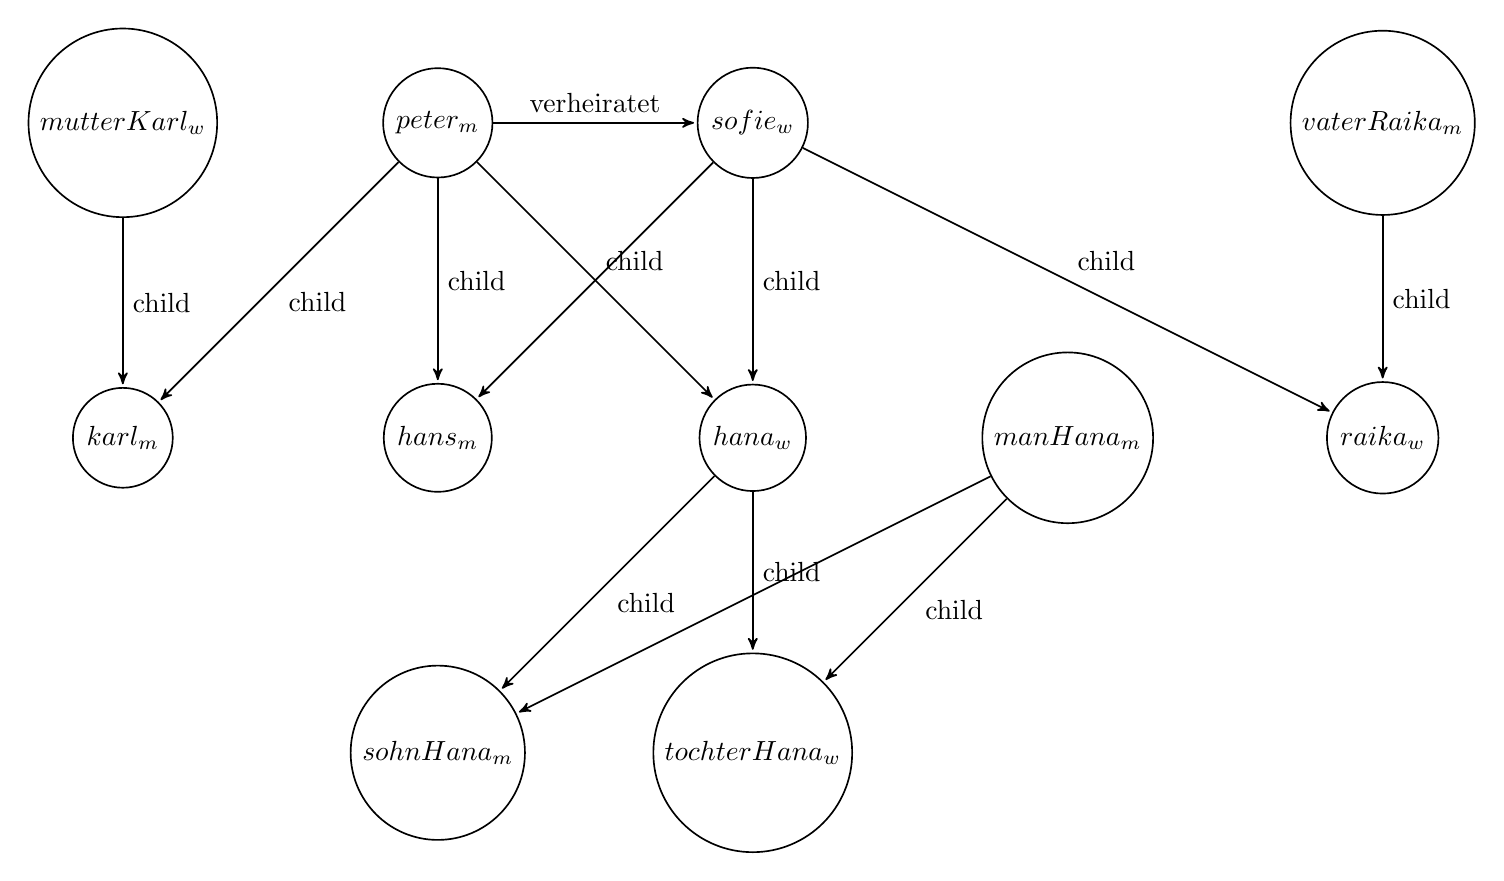
\begin{tikzpicture}[->,>=stealth',shorten >=1pt,auto,node distance=4cm,
                    semithick]
  \tikzstyle{every state}=[fill=white,draw=black,text=black]

  \node[state]			(A)                    	{$peter_m$};
  \node[state]          (B) [right of=A] 		{$sofie_w$};
  \node[state]          (C) [below of=A]		{$hans_m$};
  \node[state]          (E) [left  of=C]  		{$karl_m$};
  \node[state]          (H) [right of=C]       	{$hana_w$};
  \node[state]          (F) [right of=H]  		{$manHana_m$};
  \node[state]          (I) [left  of=A]       	{$mutterKarl_w$};
  \node[state]          (J) [right of=F]       	{$raika_w$};
  \node[state]     		(D) [above of=J] 		{$vaterRaika_m$};
  \node[state]          (K) [below of=H]       	{$tochterHana_w$};
  \node[state]          (G) [left  of=K]       	{$sohnHana_m$};

  \path (A) edge              node {verheiratet} (B)
            edge              node {child} 	(C)
			edge              node {child} 	(H)
			edge              node {child} 	(E)
		(B) edge              node {} 		(C)
			edge              node {child} 	(H)
			edge              node {child} 	(J)
		(D) edge              node {child} 	(J)
		(H) edge              node {child} 	(G)
			edge              node {child} 	(K)
		(I) edge              node {child} 	(E)
		(F) edge              node {} 		(G)
			edge              node {child} 	(K)
			;
\end{tikzpicture}

\end{document}